\begin{figure}[!h]
\centerline{\bfseries\large Low-Density Workload : Trials 1--3}\\
\fbox{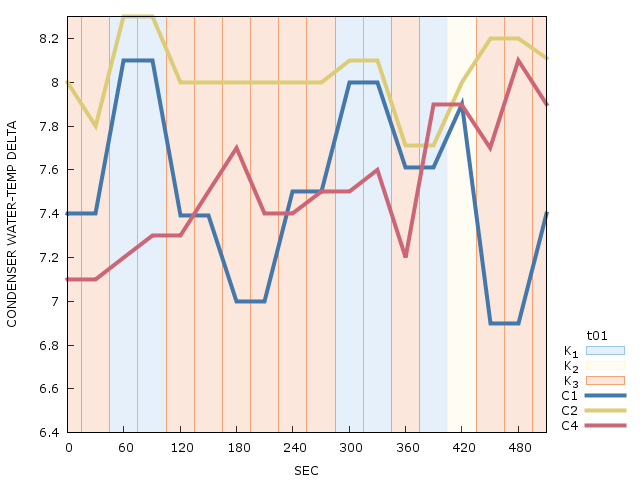
\includegraphics[bb=0 0 640 480, width=5in]{cluster3/ld/C_WTD/C_WTD_t01.png}}
\fbox{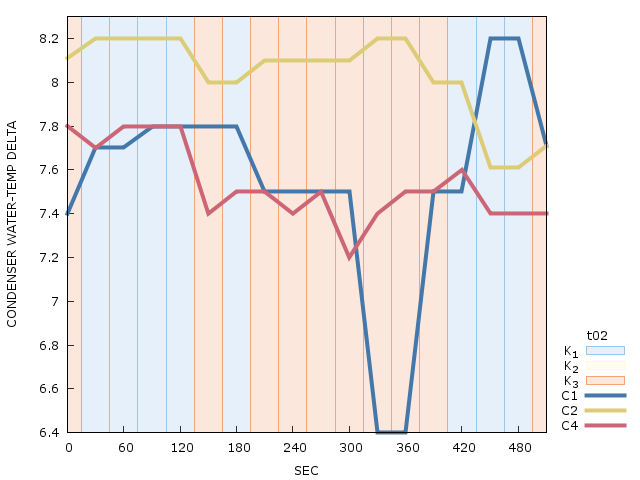
\includegraphics[bb=0 0 640 480, width=5in]{cluster3/ld/C_WTD/C_WTD_t02.png}}
\fbox{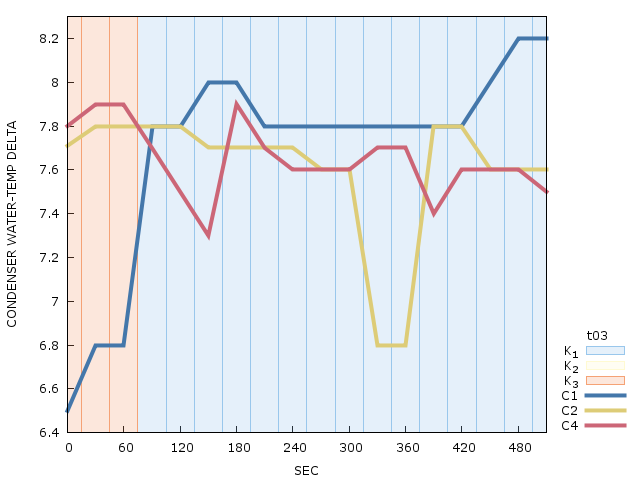
\includegraphics[bb=0 0 640 480, width=5in]{cluster3/ld/C_WTD/C_WTD_t03.png}}
\caption{Chiller units C1, C2, and C4; EM clustering across all three trials with $k=3$.}
\end{figure}
\begin{figure}[!h]
\centerline{\bfseries\large Low-Density Workload : Trials 1--3}\\
\fbox{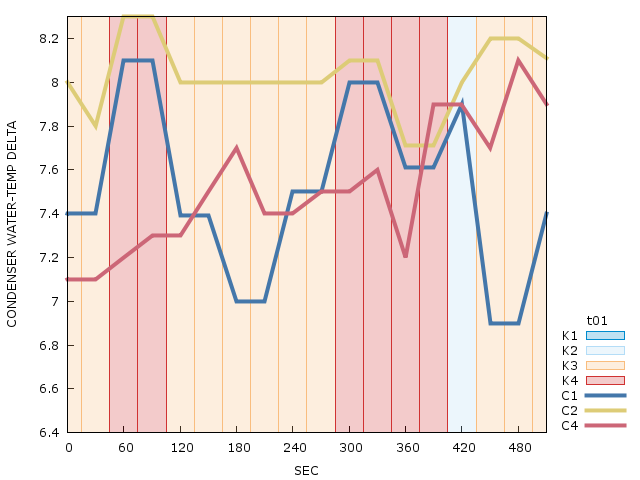
\includegraphics[bb=0 0 640 480, width=5in]{cluster4/ld/C_WTD/C_WTD_t01.png}}
\fbox{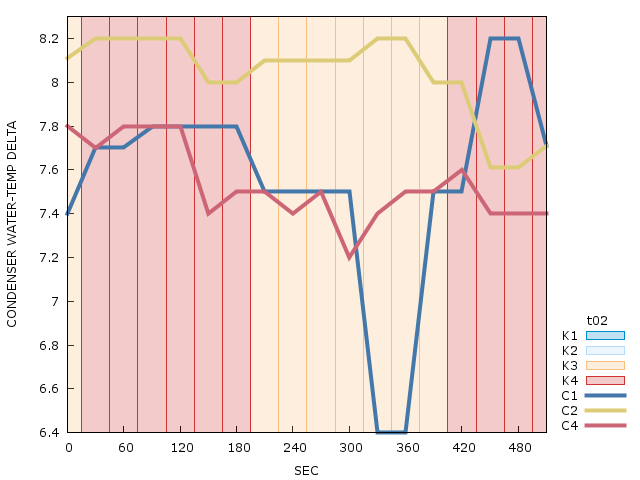
\includegraphics[bb=0 0 640 480, width=5in]{cluster4/ld/C_WTD/C_WTD_t02.png}}
\fbox{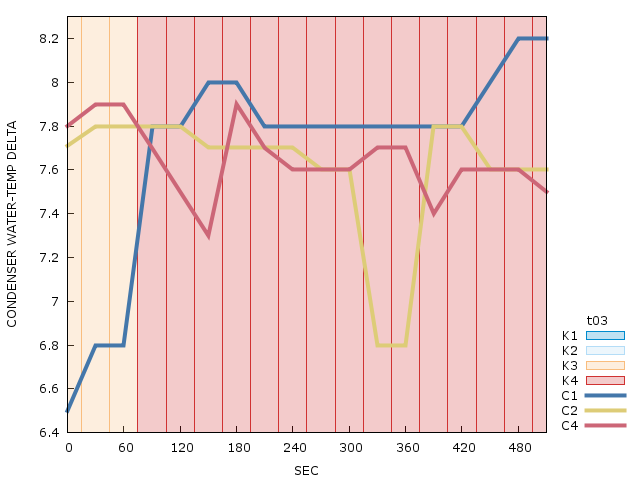
\includegraphics[bb=0 0 640 480, width=5in]{cluster4/ld/C_WTD/C_WTD_t03.png}}
\caption{Chiller units C1, C2, and C4; K-Means clustering across all three trials with $k=4$.}
\end{figure}
\begin{figure}[!h]
\centerline{\bfseries\large Low-Density Workload : Trials 1--3}\\
\fbox{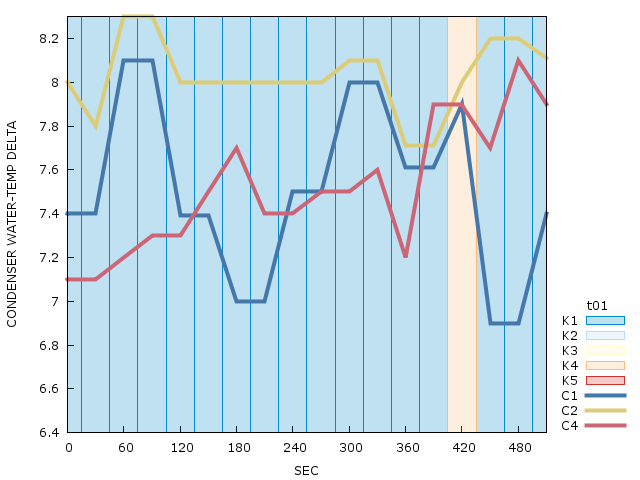
\includegraphics[bb=0 0 640 480, width=5in]{cluster5/ld/C_WTD/C_WTD_t01.png}}
\fbox{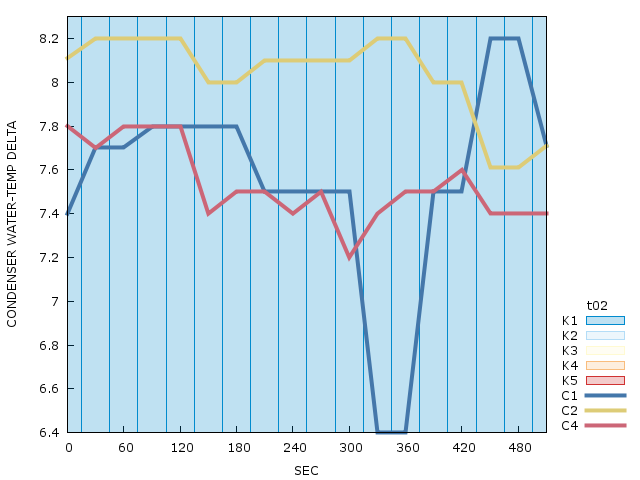
\includegraphics[bb=0 0 640 480, width=5in]{cluster5/ld/C_WTD/C_WTD_t02.png}}
\fbox{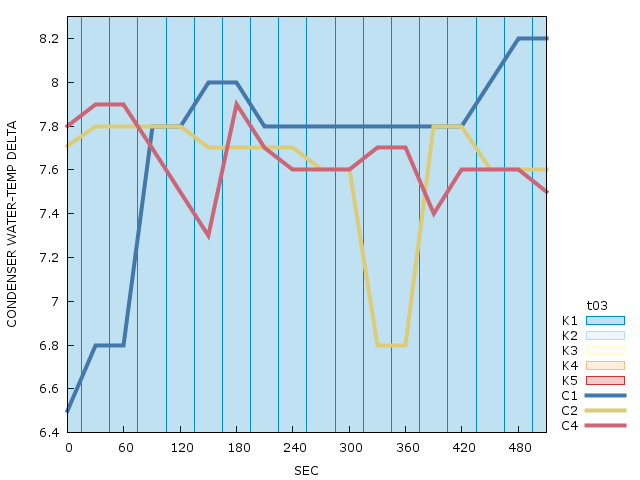
\includegraphics[bb=0 0 640 480, width=5in]{cluster5/ld/C_WTD/C_WTD_t03.png}}
\caption{Chiller units C1, C2, and C4; K-Means clustering across all three trials with $k=5$.}
\end{figure}
\begin{figure}[!h]
\centerline{\bfseries\large Low-Density Workload : Trials 1--3}\\
\fbox{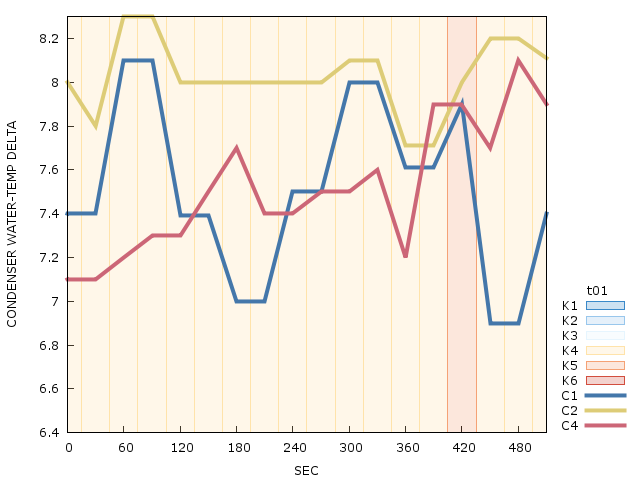
\includegraphics[bb=0 0 640 480, width=5in]{cluster6/ld/C_WTD/C_WTD_t01.png}}
\fbox{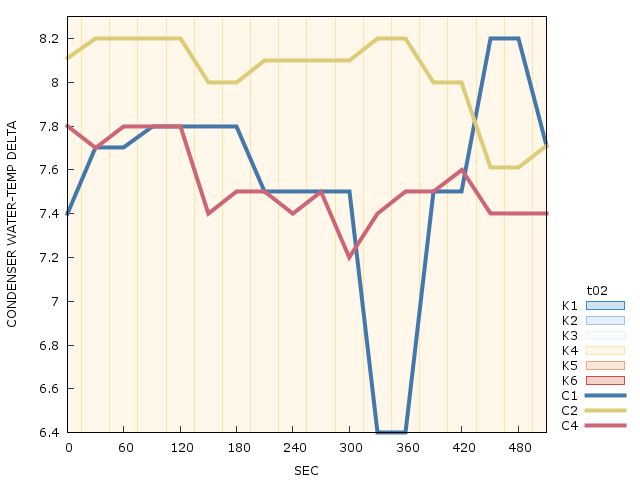
\includegraphics[bb=0 0 640 480, width=5in]{cluster6/ld/C_WTD/C_WTD_t02.png}}
\fbox{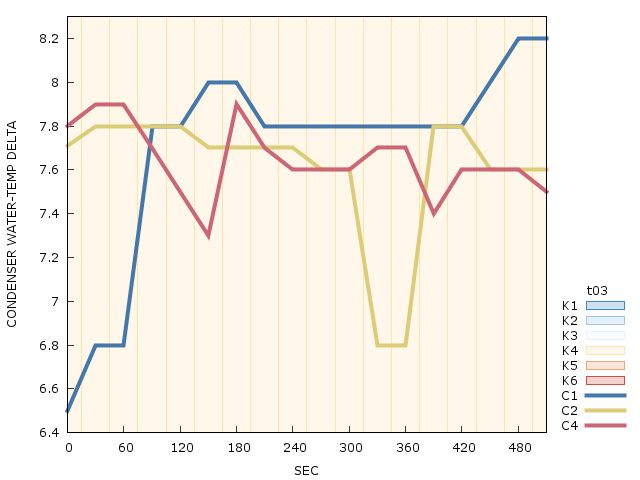
\includegraphics[bb=0 0 640 480, width=5in]{cluster6/ld/C_WTD/C_WTD_t03.png}}
\caption{Chiller units C1, C2, and C4; K-Means clustering across all three trials with $k=6$.}
\end{figure}
\begin{figure}[!h]
\centerline{\bfseries\large Low-Density Workload : Trials 1--3}\\
\fbox{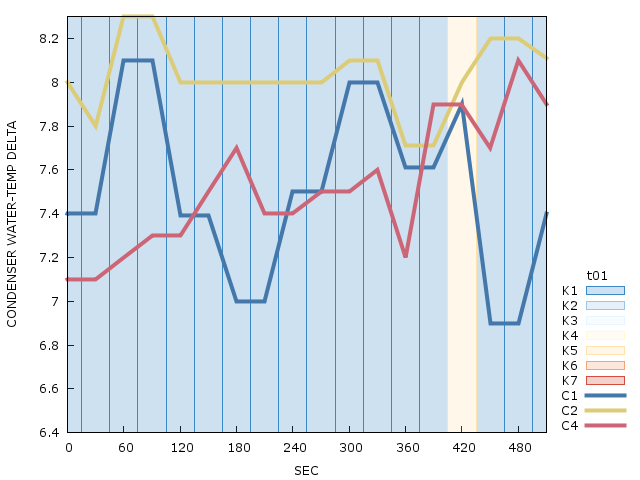
\includegraphics[bb=0 0 640 480, width=5in]{cluster7/ld/C_WTD/C_WTD_t01.png}}
\fbox{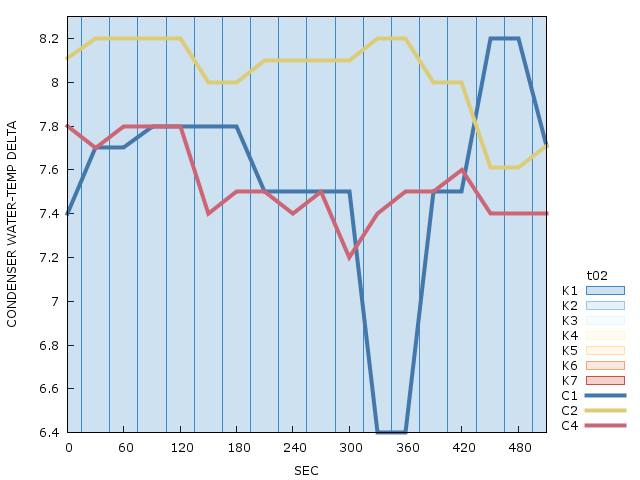
\includegraphics[bb=0 0 640 480, width=5in]{cluster7/ld/C_WTD/C_WTD_t02.png}}
\fbox{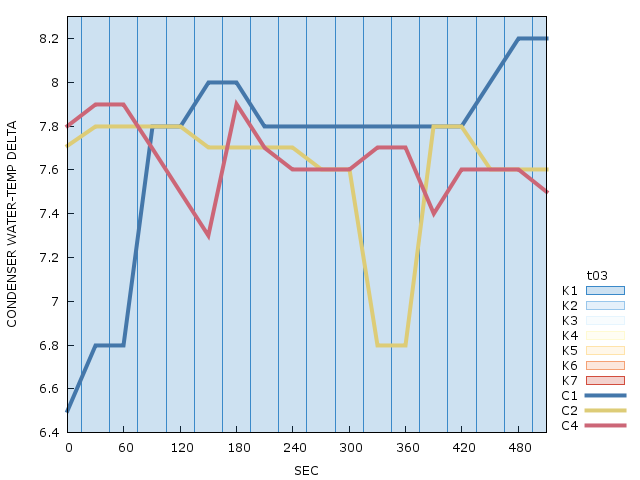
\includegraphics[bb=0 0 640 480, width=5in]{cluster7/ld/C_WTD/C_WTD_t03.png}}
\caption{Chiller units C1, C2, and C4; K-Means clustering across all three trials with $k=7$.}
\end{figure}
\begin{figure}[!h]
\centerline{\bfseries\large Low-Density Workload : Trials 1--3}\\
\fbox{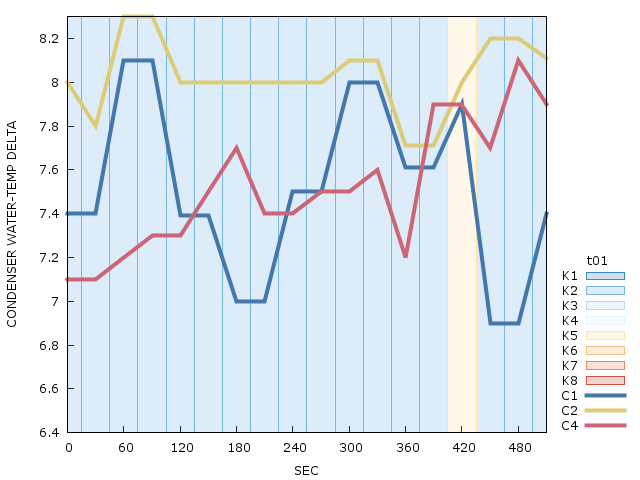
\includegraphics[bb=0 0 640 480, width=5in]{cluster8/ld/C_WTD/C_WTD_t01.png}}
\fbox{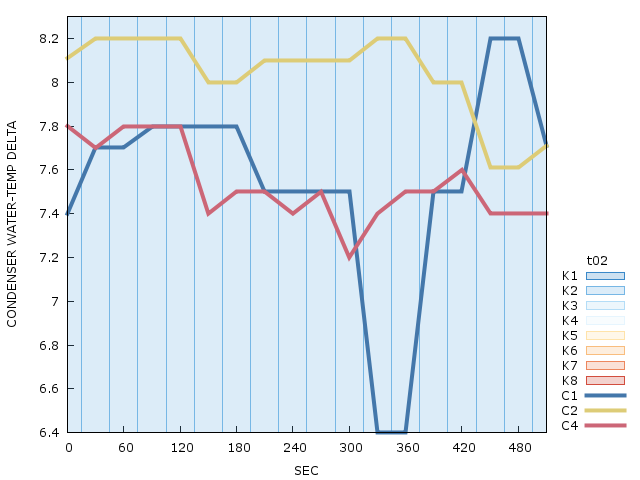
\includegraphics[bb=0 0 640 480, width=5in]{cluster8/ld/C_WTD/C_WTD_t02.png}}
\fbox{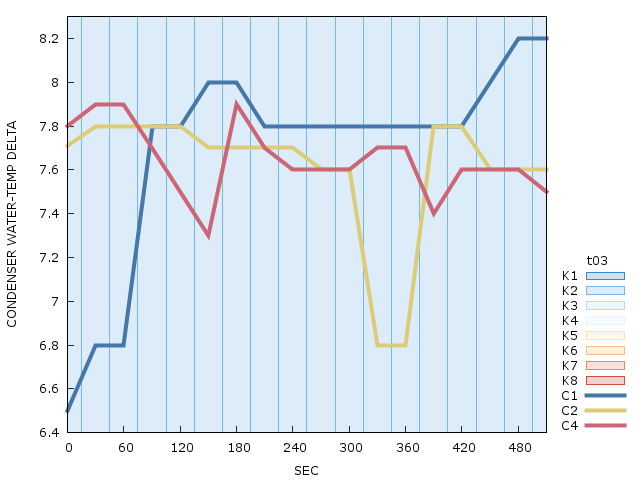
\includegraphics[bb=0 0 640 480, width=5in]{cluster8/ld/C_WTD/C_WTD_t03.png}}
\caption{Chiller units C1, C2, and C4; K-Means clustering across all three trials with $k=8$.}
\end{figure}
\begin{figure}[!h]
\centerline{\bfseries\large Low-Density Workload : Trials 1--3}\\
\fbox{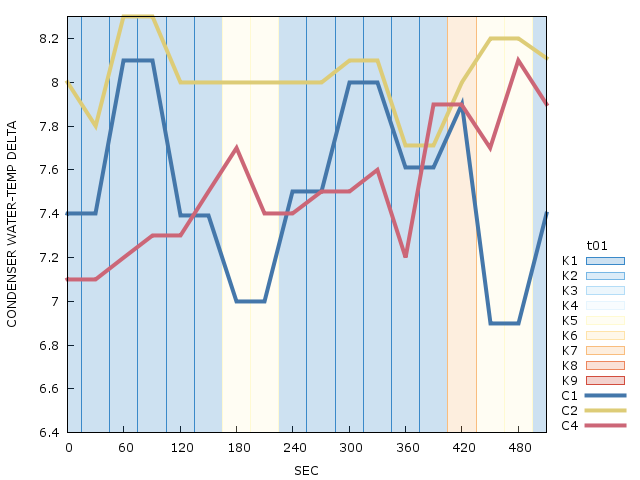
\includegraphics[bb=0 0 640 480, width=5in]{cluster9/ld/C_WTD/C_WTD_t01.png}}
\fbox{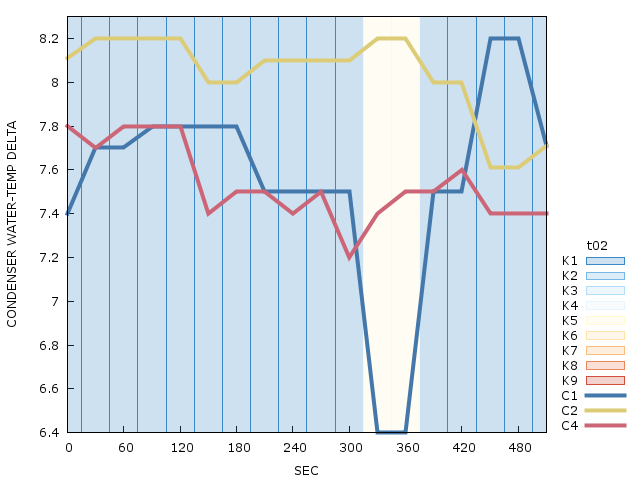
\includegraphics[bb=0 0 640 480, width=5in]{cluster9/ld/C_WTD/C_WTD_t02.png}}
\fbox{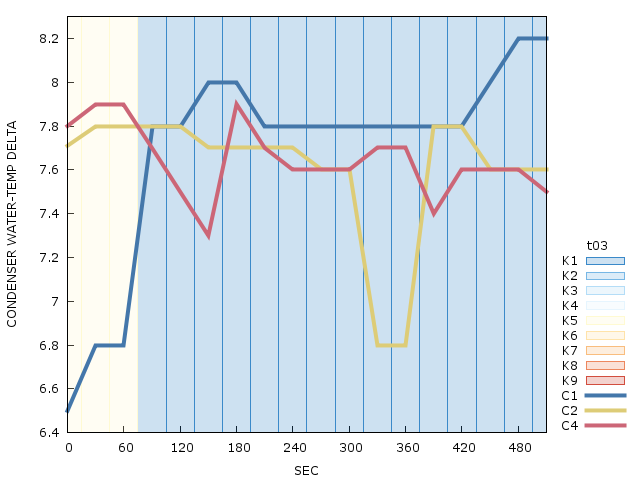
\includegraphics[bb=0 0 640 480, width=5in]{cluster9/ld/C_WTD/C_WTD_t03.png}}
\caption{Chiller units C1, C2, and C4; K-Means clustering across all three trials with $k=9$.}
\end{figure}
\begin{figure}[!h]
\centerline{\bfseries\large Low-Density Workload : Trials 1--3}\\
\fbox{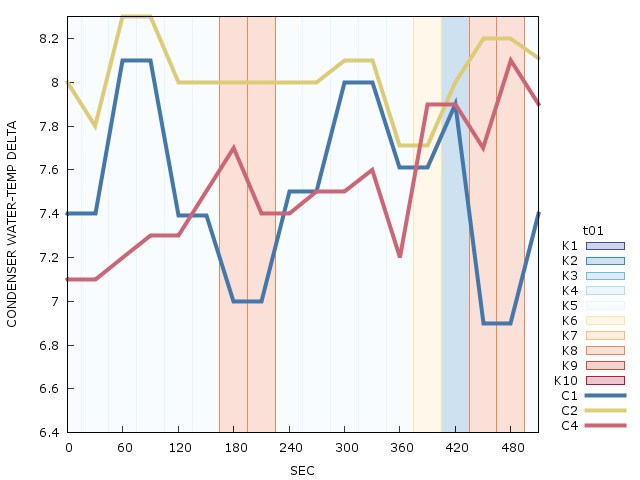
\includegraphics[bb=0 0 640 480, width=5in]{cluster10/ld/C_WTD/C_WTD_t01.png}}
\fbox{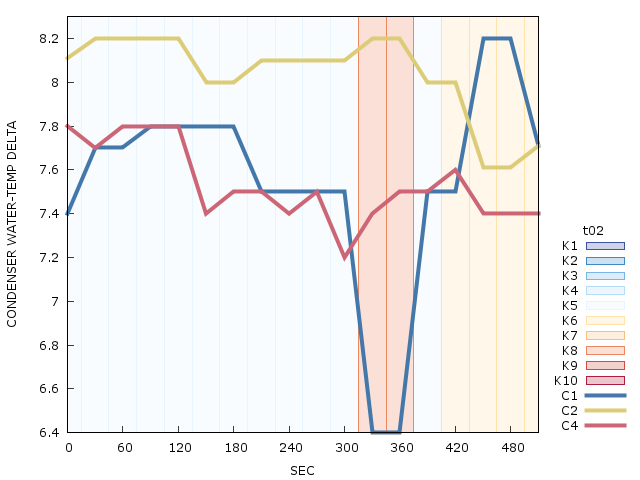
\includegraphics[bb=0 0 640 480, width=5in]{cluster10/ld/C_WTD/C_WTD_t02.png}}
\fbox{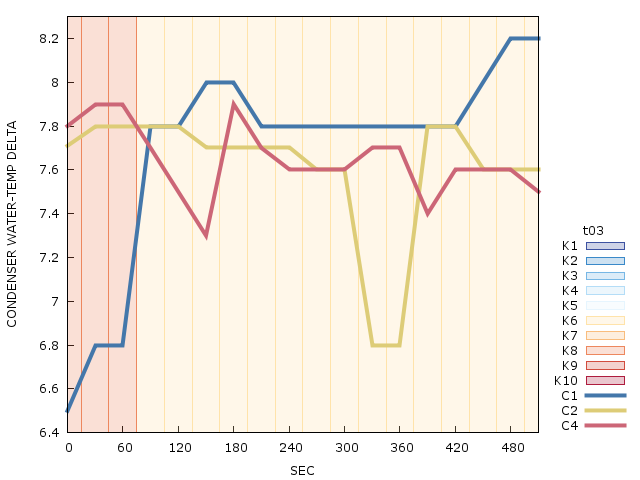
\includegraphics[bb=0 0 640 480, width=5in]{cluster10/ld/C_WTD/C_WTD_t03.png}}
\caption{Chiller units C1, C2, and C4; K-Means clustering across all three trials with $k=10$.}
\end{figure}
\begin{figure}[!h]
\centerline{\bfseries\large Low-Density Workload : Trials 1--3}\\
\fbox{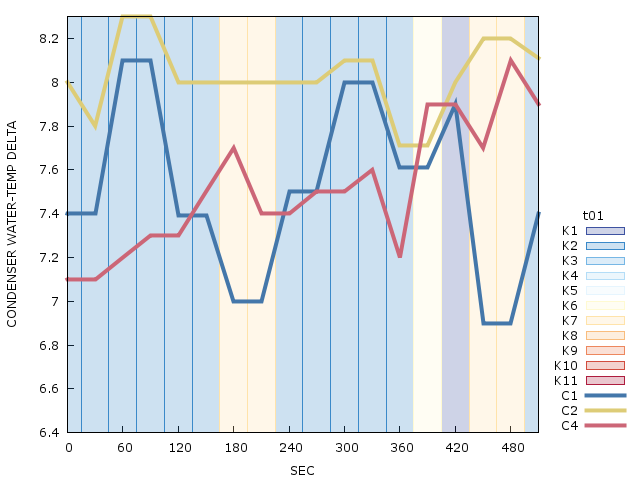
\includegraphics[bb=0 0 640 480, width=5in]{cluster11/ld/C_WTD/C_WTD_t01.png}}
\fbox{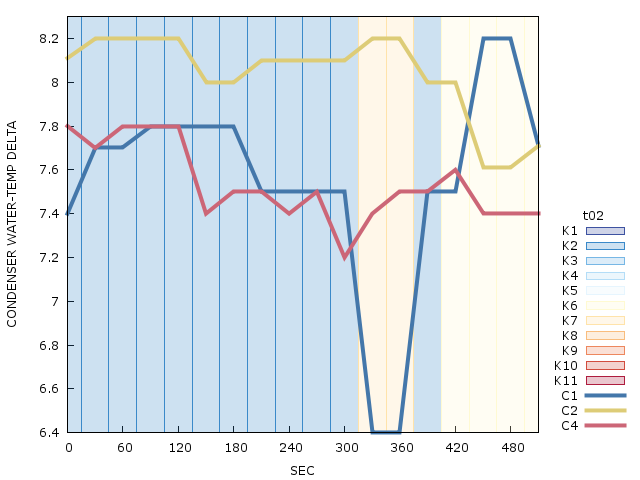
\includegraphics[bb=0 0 640 480, width=5in]{cluster11/ld/C_WTD/C_WTD_t02.png}}
\fbox{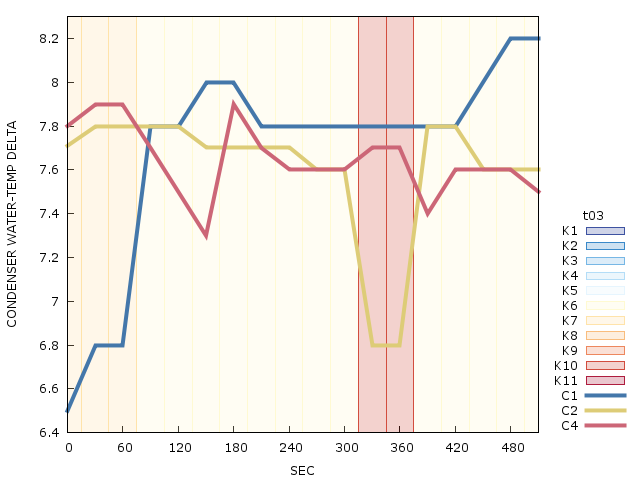
\includegraphics[bb=0 0 640 480, width=5in]{cluster11/ld/C_WTD/C_WTD_t03.png}}
\caption{Chiller units C1, C2, and C4; K-Means clustering across all three trials with $k=11$.}
\end{figure}
